\begin{figure}[H]
    \centering
    \begin{subfigure}[t]{.45\textwidth}
    \centering
    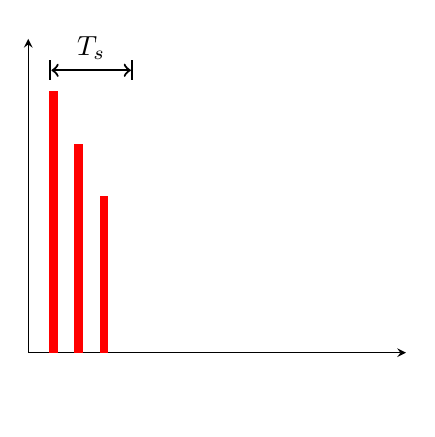
\begin{tikzpicture}
    \begin{axis}[
        axis lines=left,
        scale=0.7,
        xmin=0,xmax=3,
        ymin=0,ymax=3,
        ticks=none,
        clip=false,
    ]
    \addplot[ycomb,red,line width=3pt] plot coordinates {
        (0.2,2.5)
        (0.4,2.0)
        (0.6,1.5)
    };

    \draw[|<->|,thick] ([xshift=-1.5pt]axis cs:0.2,2.7) -- ([xshift=+1.5pt]axis cs:0.8,2.7) node[midway,above] {$T_s$};

    \path ([xshift=-1.5pt]axis cs:0.2,-.2) -- ([xshift=+1.5pt]axis cs:0.6,-.2) node[midway,below,text opacity=0] {$\tau_1$};
    \end{axis}
    \end{tikzpicture}
    \caption{Flat fading channel.}
    \label{fig:flat}
    \end{subfigure}
    \begin{subfigure}[t]{.45\textwidth}
    \centering
    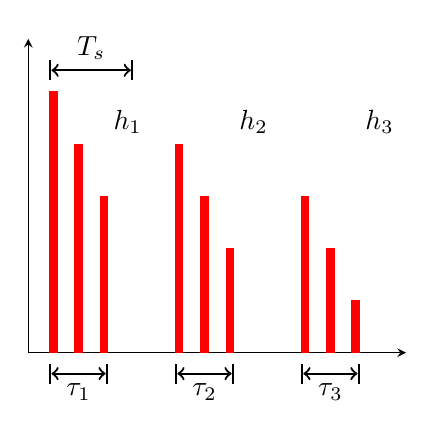
\begin{tikzpicture}
    \begin{axis}[
        axis lines=left,
        scale=0.7,
        xmin=0,xmax=3,
        ymin=0,ymax=3,
        ticks=none,
        clip=false,
    ]
    \addplot[ycomb,red,line width=3pt] plot coordinates {
        (0.2,2.5)
        (0.4,2.0)
        (0.6,1.5)
    };

    \addplot[ycomb,red,line width=3pt] plot coordinates {
        (1.2,2.0)
        (1.4,1.5)
        (1.6,1.0)
    };

    \addplot[ycomb,red,line width=3pt] plot coordinates {
        (2.2,1.5)
        (2.4,1.0)
        (2.6,0.5)
    };

    \draw[|<->|,thick] ([xshift=-1.5pt]axis cs:0.2,2.7) -- ([xshift=+1.5pt]axis cs:0.8,2.7) node[midway,above] {$T_s$};

    \draw[|<->|,thick] ([xshift=-1.5pt]axis cs:0.2,-.2) -- ([xshift=+1.5pt]axis cs:0.6,-.2) node[midway,below] {$\tau_1$};

    \draw[|<->|,thick] ([xshift=-1.5pt]axis cs:1.2,-.2) -- ([xshift=+1.5pt]axis cs:1.6,-.2) node[midway,below] {$\tau_2$};

    \draw[|<->|,thick] ([xshift=-1.5pt]axis cs:2.2,-.2) -- ([xshift=+1.5pt]axis cs:2.6,-.2) node[midway,below] {$\tau_3$};

    \node[anchor=south west] at (axis cs:0.6,2.0) {$h_1$};

    \node[anchor=south west] at (axis cs:1.6,2.0) {$h_2$};

    \node[anchor=south west] at (axis cs:2.6,2.0) {$h_3$};
    \end{axis}
    \end{tikzpicture}
    \caption{Frequency selective channel.}
    \label{fig:freq}
    \end{subfigure}
    \caption{Different channel types.}
    \label{fig:channels}
\end{figure}
